\documentclass[a4paper, 12pt, final, garamond]{book}
\usepackage{cours-preambule}
\graphicspath{{../figures/}}

\raggedbottom

\makeatletter
\renewcommand{\@chapapp}{Programme de kh\^olle -- semaine}
\makeatother

\begin{document}
\setcounter{chapter}{12}

\chapter{Du 08 au 11 janvier}

\section{Cours et exercices}
\ssubsection{E7}{Filtrage linéaire}
\begin{enumerate}[label=\Roman*]
	\bitem{Signaux périodiques}~: période, moyenne, valeur efficace.
	\bitem{Décomposition en série de Fourier}~: théorème de
	\textsc{Fourier}, analyse spectrale, relation de \textsc{Parseval}.
	\bitem{Filtrage linéaire}~: introduction, fonction de transfert d'un
	filtre, effet d'un filtre sur un signal périodique.
	\bitem{Description d'un filtre}~: gain et gain en décibels, diagramme
	de \textsc{Bode} (définition, exemple, asymptotes, lecture), filtres
	moyenneurs dérivateurs et intégrateurs.
	\bitem{Filtres d'ordre 1}~: RC sur C~: passe-bas, RC sur R~:
	passe-haut.
	\bitem{Filtres d'ordre 2}~: RLC sur C~: passe-bas d'ordre 2, RLC sur R~:
	passe-bande.
	\bitem{Filtres en cascade}~: nécessité d'adaptation d'impédance.
\end{enumerate}

\ssubsection{ON1}{Ondes progressives}
\begin{enumerate}[label=\Roman*]
	\bitem{Introduction}~: signal, perturbation, onde, propagation.
	\bitem{Onde progressive à une dimension}~: définition, représentation
	spatiale, célérité, représentation temporelle, retard, lien entre les
	représentations, formes mathématiques.
	\bitem{Onde progressive sinusoïdale}~: définition, double
	périodicité, rappel spectre électromagnétique, expression mathématique
	de l'OPS, vitesse de phase.
	\bitem{Milieux dispersifs}~: définition, exemples.
\end{enumerate}

\section{Cours uniquement}
\ssubsection{ON2}{Interférences à deux ondes}
\begin{enumerate}[label=\Roman*]
	\bitem{Rappel déphasages}~: définition, valeurs particulières,
	lecture graphique.
	\bitem{Superposition d'ondes sinusoïdales de mêmes fréquences}~:
	introduction, signaux de même amplitude, signaux d'amplitudes
	différentes, bilan.
	\bitem{Approximation par une onde plane}~: sources ponctuelles,
	différence de marche, exercice d'application.
	\bitem{Interférences lumineuses}~: cohérence, intensité, formule de
	\textsc{Fresnel}, chemin optique.
	\bitem{Expérience des trous d'\textsc{Young}}~: introduction,
	présentation, détermination de l'interfrange.
\end{enumerate}

\newpage

\section{Questions de cours possibles}
\ssubsection{E7}{Filtrage linéaire}
\begin{enumerate}
	\item Pour un des filtres ci-dessous~: présenter le système réel, le système
	      en RSF, déterminer sa fonction de transfert, son gain en décibels, son
	      déphasage, déterminer les asymptotes et tracer les diagrammes de
	      \textsc{Bode}.
	      \begin{tasks}(4)
		      \task RC sur C
		      \task RC sur R
		      \task RLC sur C
		      \task RLC sur R
	      \end{tasks}
	\item Définir les trois effets de filtres étudiés~: moyenneur, intégrateur
	      dérivateur. Donner les formes canoniques des filtres passe-bas et passe-haut
	      d'ordre 1 et démontrer leur comportement intégrateur ou dérivateur.
	      Représentez l'effet d'un intégrateur sur un signal créneau et l'effet d'un
	      intégrateur sur un signal triangle.
\end{enumerate}
\ssubsection{ON1}{Ondes progressives}
\begin{enumerate}[resume]
	\item On considère ici un mascaret qui se déplace à la vitesse $c =
		      \SI{18}{km.h^{-1}}$ le long d'un fleuve rectiligne, et on définit un axe
	      $(Ox)$ dans la direction du sens de sa propagation.

	      À l'instant $t=0$, le profil du niveau de l'eau du fleuve a l'allure
	      suivante~:
	      \begin{center}
		      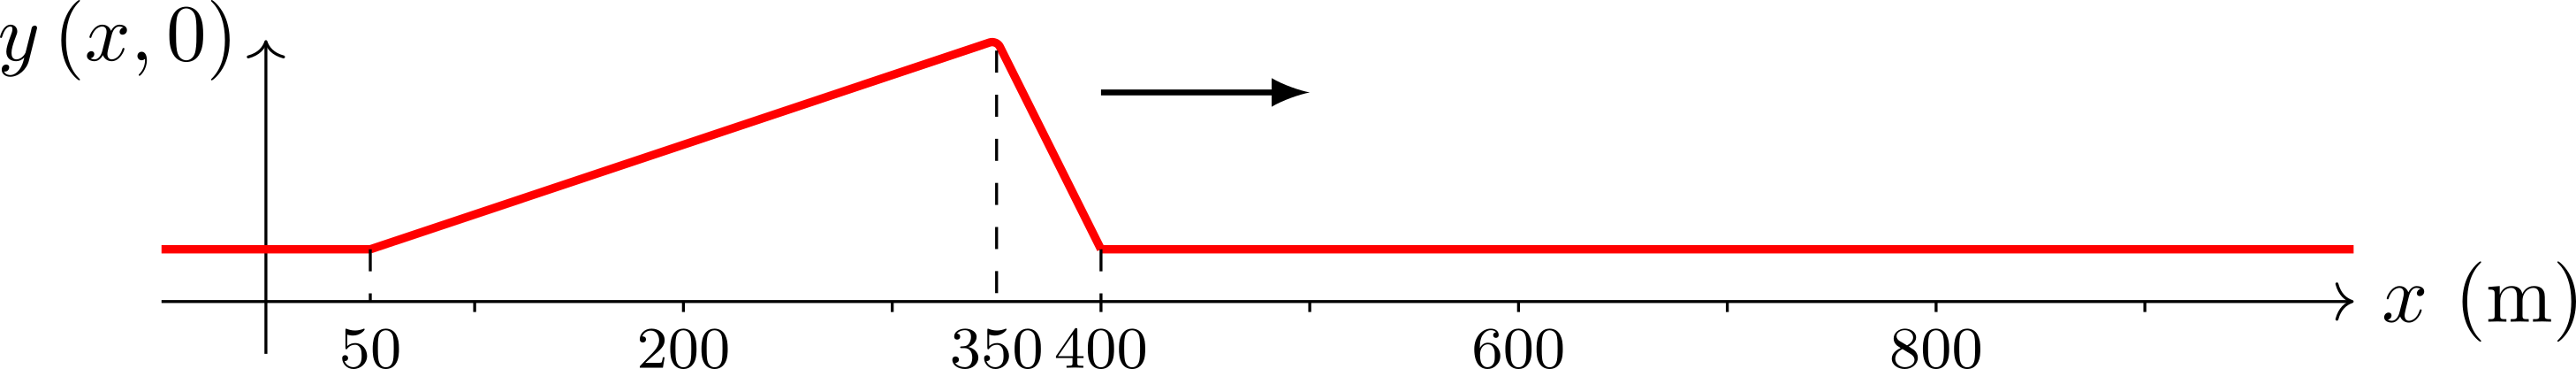
\includegraphics[width=0.8\linewidth]{rep_spa-masc_a}
	      \end{center}
	      \begin{enumerate}[label=\sqenumi]
		      \item Faire un schéma du profil du fleuve à $\tau = \SI{1}{min}$ en
		            supposant que l'onde se propage sans déformation.
		      \item À quel instant la vague arrive-t-elle au point d'abscisse $x_1 =
			            \SI{2.2}{km}$~?
		      \item Un détecteur fixe, enregistrant la hauteur du fleuve en fonction
		            du temps, est placé à l'abscisse $x_d = \SI{1.6}{km}$. Dessiner
		            l'allure des variations $y(x_d,t)$ en fonction du temps à cette
		            abscisse.
	      \end{enumerate}
	\item Présenter ce qu'est une onde progressive sinusoïdale, établir sa
	      double périodicité, indiquer les différentes relations reliant $\omega$
	      et $f$ ou $T$~; $k$ et $\lambda$~; $\lambda$, $c$ et $f$ ou $T$. Définir
	      un milieu dispersif et donner des exemples.
	\item Répondre à au moins 2 questions parmi les suivantes (nombre au choix
	      de l'interrogataire)~:
	      \begin{enumerate}
		      \item Soit $f(t)$ la fonction modélisant un signal en $x=0$. Donner
		            et démontrer l'expression du signal $s(x,t)$ en M$(x)$ ($x>0$) en
		            considérant une onde qui se propage vers les $x$ croissants de O à
		            M à la célérité $c$ en fonction de $f$.

		      \item Soit $f(t)$ la fonction modélisant un signal en $x=0$. Donner
		            et démontrer l'expression du signal $s (x,t)$ en M$(x)$ ($x<0$) en
		            considérant une onde qui se propage vers les $x$ décroissants de O
		            à M à la célérité $c$ en fonction de $f$.

		      \item Soit $g(x)$ la fonction modélisant un signal en $t=0$. Donner
		            et démontrer l'expression du signal $s (x,t)$ en M$(x)$ ($x<0$) en
		            considérant une onde se propageant vers les $x$ décroissants à la
		            célérité $c$ en fonction de $g$.

		      \item Une onde progressive sinusoïdale d'amplitude $A_0$ et de
		            longueur d'onde $\lambda$ se propage dans le sens des $x$
		            décroissants à la célérité $c$. La phase à $t=0$ au point A
		            d'abscisse $x_A = {\lambda}/{4}$ est nulle. Donner l'expression
		            de la fonction $s(x,t)$ en fonction de $A_0$, $\lambda$, $c$,
		            $x$ et $t$. Quel est le déphasage entre A et l'origine O du
		            repère~?

		      \item Une onde sinusoïdale se propage dans la direction de l'axe
		            $(Ox)$ dans le sens négatif avec la célérité $c$. On donne~:
		            \hfill
		            $\boxed{s_2(0,t) = A \sin(\omega t)}$
		            \hfill~
		            \smallbreak
		            Déterminer l'expression de $s_2(x,t)$. Représenter graphiquement
		            $s_2(\lambda/4,t)$ et $s_2(\lambda/2,t)$ en fonction de $t$.
	      \end{enumerate}
\end{enumerate}

\ssubsection{ON2}{Interférences à deux ondes}
\begin{enumerate}[resume]
	\item Déterminer l'expression du signal somme de deux ondes sinusoïdales de
	      même fréquence \textbf{et même amplitude} en introduisant $\Delta
		      \f_{1/2}(\Mr)$ et $\f_0(\Mr)$. On rappelle la formule de trigonométrie
	      \[
		      \cos p + \cos q =
		      2\cos \left( \frac{p+q}{2} \right)\cos \left( \frac{p-q}{2} \right)
	      \]
	      Décrire le signal obtenu. Détailler les
	      cas extrêmes et les valeurs de déphasage correspondantes (on utilisera
	      l'ordre d'interférence et non la congruence). Qu'est-ce qui change si
	      les signaux n'ont pas la même amplitude~? Définir les termes
	      d'interférences constructives et destructives.
	\item Démontrer le lien entre déphasage et différence de marche. Expliquer
	      avec vos mots ce que représente la différence de marche. Démontrer les
	      valeurs de différence de marche correspondant aux situations de signaux en
	      phase et en opposition de phase. Définir et démontrer le chemin optique
	      d'un rayon lumineux, et donner le lien entre entre déphasage et chemin
	      optique.
	\item
	      Soient 2 émetteurs sonores envoyant une onde progressive sinusoïdale de
	      même fréquence, amplitude et phase à l'origine. Le premier est fixé à
	      l'origine du repère, l'émetteur 2 est mobile et à une distance $d$ du
	      premier, et un microphone est placé à une distance fixe $x_0$ de
	      l'émetteur 1 et est aligné avec les deux émetteurs. On néglige
	      l'influence de l'émetteur 2 sur l'émetteur 1 et toute atténuation.
	      \begin{enumerate}[label=\sqenumi]
		      \item Faire un schéma.
		      \item Lorsque $d=0$, qu'enregistre-t-on au niveau du microphone~?
		      \item On part de $d=0$ et on augmente $d$ jusqu'à ce que le signal
		            enregistré soit nul. Ceci se produit pour $d = \SI{6.0}{cm}$.
		            Expliquer cette extinction.
		      \item En déduire la longueur d'onde du son émis.
		      \item Pour $d = \SI{12.0}{cm}$, quelle sera l'amplitude du signal
		            enregistré~?
	      \end{enumerate}
	\item Expliquer ce qu'est la cohérence et pourquoi on ne fait des interférence
	      qu'avec une unique source pour des signaux lumineux. Définir ce qu'est
	      l'intensité d'un signal. Démontrer la formule de
	      \textsc{Fresnel} pour deux signaux sinusoïdaux de même fréquence et
	      d'amplitudes différentes. La simplifier pour des signaux de même amplitude.
	\item Trous d'\textsc{Young}~: présenter l'expérience et montrer que la
	      différence de chemin $\delta_{2/1}(\Mr)$ s'écrit \hfill $\delta =
		      2ax/D$ avec $2a$ la distance entre les fentes. Donner les conditions sur
	      $x$ pour avoir interférences constructives ou destructives.
	      \smallbreak
	      On donne le développement limité suivant~:
	      \[\sqrt{1+\ep} = 1 + \ep/2 + o(\ep)\]
\end{enumerate}


\end{document}
